\documentclass{ieeeaccess}
\usepackage{cite}
\usepackage{amsmath,amssymb,amsfonts}
\usepackage{algorithmic}
\usepackage{graphicx}
\usepackage{textcomp}
\usepackage{mathtools}
\usepackage[pdftex]{graphicx}

\usepackage{tensor}
\usepackage{booktabs}
\usepackage{url}
\usepackage{diagbox}
\usepackage{setspace}
\usepackage{threeparttable}
\newcommand{\degree}{^\circ}

\def\BibTeX{{\rm B\kern-.05em{\sc i\kern-.025em b}\kern-.08em
    T\kern-.1667em\lower.7ex\hbox{E}\kern-.125emX}}
\begin{document}
\history{Date of publication xxxx 00, 0000, date of current version xxxx 00, 0000.}
\doi{10.1109/ACCESS.2017.DOI}

\title{QR code-based self-calibration for a fault-tolerant industrial robot arm}
\author{\uppercase{Yizheng Zhang}\authorrefmark{1},
\uppercase{Wangshu Zhu\authorrefmark{2}, and Andre Rosendo}\authorrefmark{3}}
\address[1]{
	Living Machine Lab,
	ShanghaiTech University,
	Shanghai, China
	(e-mail: zhangyzh1@shanghaitech.edu.cn)}
\address[2]{
	Living Machine Lab,
ShanghaiTech University,
Shanghai, China
(e-mail: zhuwsh@shanghaitech.edu.cn)}
\address[3]{
	Living Machine Lab,
ShanghaiTech University,
Shanghai, China
(e-mail: arosendo@shanghaitech.edu.cn)}
%\tfootnote{This paragraph of the first footnote will contain support 
%information, including sponsor and financial support acknowledgment. For 
%example, ``This work was supported in part by the U.S. Department of 
%Commerce under Grant BS123456.''}

\markboth
{Author \headeretal: Preparation of Papers for IEEE TRANSACTIONS and JOURNALS}
{Author \headeretal: Preparation of Papers for IEEE TRANSACTIONS and JOURNALS}

\corresp{Corresponding author: Yizheng Zhang(e-mail: zhangyzh1@shanghaitech.edu.cn).}

\begin{abstract}
	Malfunctions on industrial robots can cost factories 22,000 dollars per minute. Although the benefits of a fault-tolerant robot arm are clear, redundant sensors would steeply add to the costs of such robots, while machine learning-based methods spend too much time learning the robot's model. We propose a simple but high effective method to infer which joint underwent failure and at which angle this joint is constrained, to then modify the inverse kinematics (IK) algorithm to adaptively achieve the goal. Our method involves combining a QR code with an inexpensive camera, building a virtual link between these two to give the relative position of the end effector. Once one joint/encoder/motor suffers damage, we use this virtual link to calibrate this joint by coordinate transformation, to calculate the constrained angle, and to recalculate the trajectory through IK iterations with the Newton-Raphson method. We prove the efficacy of our method with pick-and-place experiments, commonly seen in industrial settings, emulating malfunctions on different joints and at different angles, and our method can successfully finish the task in most cases. We further demonstrate that our method is capable, for almost all of the six degree-of-freedom manipulators, to adapt to joint failures after suffering a position failure. With the steep increase of robots within factories this work presents an elegant approach to keep robots functional until maintenance is scheduled, reducing downtime.
%These instructions give you guidelines for preparing papers for 
%IEEE Access. Use this document as a template if you are 
%using \LaTeX. Otherwise, use this document as an 
%instruction set. The electronic file of your paper will be formatted further 
%at IEEE. Paper titles should be written in uppercase and lowercase letters, 
%not all uppercase. Avoid writing long formulas with subscripts in the title; 
%short formulas that identify the elements are fine (e.g., "Nd--Fe--B"). Do 
%not write ``(Invited)'' in the title. Full names of authors are preferred in 
%the author field, but are not required. Put a space between authors' 
%initials. The abstract must be a concise yet comprehensive reflection of 
%what is in your article. In particular, the abstract must be self-contained, 
%without abbreviations, footnotes, or references. It should be a microcosm of 
%the full article. The abstract must be between 150--250 words. Be sure that 
%you adhere to these limits; otherwise, you will need to edit your abstract 
%accordingly. The abstract must be written as one paragraph, and should not 
%contain displayed mathematical equations or tabular material. The abstract 
%should include three or four different keywords or phrases, as this will 
%help readers to find it. It is important to avoid over-repetition of such 
%phrases as this can result in a page being rejected by search engines. 
%Ensure that your abstract reads well and is grammatically correct.
\end{abstract}

\begin{keywords}
Fault tolerance,Self Calibration, Adaptive Robotics, QR Code, Robot Arm;
\end{keywords}

\titlepgskip=-15pt

\maketitle

\section{Introduction}
\label{sec:introduction}
\PARstart{M}{alfunctions} on rotary encoders or electric motors within an industrial manipulator can cause great losses for factories. 
Long-term work hours increase the tendency of robot arms to suffer various faults.
These faults not only shorten manipulators service life, but also make them unable to perform scheduled tasks in the factory, which may even lead to catastrophic consequences. 
Fault-tolerance is the property that enables a system to continue operating properly in the event of a failure in some of its components, and this property is very important when robot arms are needed to perform tasks in complex and unknown environments, like space applications.


%%%%%%%%%%%%%%%%%%%%%%%%
Manipulator faults can be divided into the following three types:

1. Free swinging failure \cite{english1998fault,english2000measuring},  due to the actuator not being capable of actively exert any torque (or force). Another name is torque failure. 

2. Position failure, which acts as if the actuator was locked \cite{maciejewski1990fault,paredis1994kinematic,roberts1996local}, i.e., the joint cannot change its angle or length.

3. Sensor failure \cite{english2000measuring},
where the joint value is perturbed by an unknown,
possibly time-varying, value. 
%
%These failures all eventually
%express themselves through joint position error. Errors may
%involve multiple joints (as, for example, when a hydraulic
%system loses pressure), but it is typical—and is assumed for this
%work—that a failure-induced error is isolated to one joint. This
%joint error is an imprecise measure of the effect of the failure,
%however, even for the same joint on the same manipulator.
%
%1. locking , joint cannot move (another expression: position failure)\cite{maciejewski1990fault,paredis1994kinematic,roberts1996local}
%I  these three paper because this paper\cite{english2000measuring} cite these three
%2. free swing(another expression: torque failure) 
% free swinging, where actuator torque is lost 
%\cite{english1998fault,english2000measuring}I cite these two paper because this paper\cite{chen2003optimal} cite these two.
%
%3. calibration, (another expression:Sensor fault) 
%where the joint value is perturbed by an unknown,
%possibly time-varying, value. 
%These failures all eventually
%express themselves through joint position error. Errors may
%involve multiple joints (as, for example, when a hydraulic
%system loses pressure), but it is typical—and is assumed for this
%work—that a failure-induced error is isolated to one joint. This
%joint error is an imprecise measure of the effect of the failure,
%however, even for the same joint on the same manipulator. 
%
%measured in Euclidean space!

%%%%%%%%%%%%%%%%%%%%%%%%

To the best of our knowledge, there are mainly two approaches for robots to adapt to malfunctions: model-based and learning-based. Works such as the one presented by \cite{goel2005analyzing} tackles the problem from a mathematical perspective, while others, such as \cite{7832455}, \cite{cully2015robots} and \cite{chatzilygeroudis2017black} use heuristics to converge to a solution.

From a model-based perspective, Goel et al. \cite{goel2005analyzing} focus on a case where one of the joints is locked but the controller continues to control that joint as though it were healthy. For a general class of tasks characterized by point-to-point motion, they examine convergence issues such as whether the manipulator comes to rest and, if so, what is the terminal position and orientation of the end-effector. Their application is limited, as they only consider joint position failure, which means that they already know the constrained angle value. On the other hand, Filion et al. \cite{filion2018robot} and Hefele et al.\cite{hefele2001robot} focus on photogrammetry way by using a high resolution camera. But their methods take extra space and the devices can be expensive. Also, \cite{hefele2001robot} has a high requirement for environment to achieve a robust target identification and precise measurement.

%We both assume that joint failure and sensor failure. But they focus on convergence issues and try to solve from convergence issues. But we rebuild our kinematic chain. Their model is complex when it become three dimension, but ours is simple.

A great body of research has been combining learning algorithms with robotics, and some focus on applications on robot manipulators: Jutharee and Maneewarn \cite{7832455} use a Genetic Algorithm optimization method to the 7 degree-of-freedom (DOF) of a semi-humanoid robot when a joint failure occurred. However, similarly to \cite{goel2005analyzing}, their work assumes that the constrained angle value is known.

%We consider both joint failure and sensor failure. It looks work well on reception robot but may not work for industrial manipulator due to the high precision requirement. 

More recently, Cully et al.\cite{cully2015robots} developed a hexapod robot and a manipulator that can adapt its behavior after a malfunction by using a method called Intelligent Trial and Error (IT\&E) algorithm. While IT\&E is a combination of a simulation-based Genetic Algorithm parametric search with a Bayesian Optimization real-world heuristic, there is no knowledge of what the fault or optimum behavior is. In their data-driven approach their manipulator requires a few iterations to converge to a working solution, and in recent works the same authors propose a variant of the same algorithm for a policy-search within a Reinforcement Learning problem on a 4 DOF manipulator \cite{chatzilygeroudis2017black}. Although this work shows a remarkable performance, converging to an optimal solution within 35 seconds of iteration time, the computational time spent between iterations is very high. Additionally, the need for trials to converge to a working solution is far from desirable within industrial settings.
%We are model-based and our method is highly accurate and industrial manipulator need high precision. The way to measure its performance can be various from one robot to other robot. But we are easy to deploy and highly compatible.

In our work, we propose a simple and inexpensive method to overcome both position failure and sensor failure. We use a QR code to build a virtual link to estimate the transformation matrix between the two adjacent links, to calibrate the constrained angle and lastly to plan a new trajectory. We then draw a comparison between our work and previous works from other researchers, and discuss the range of applications where model-based and data-driven approaches can be used. This work (to the best of our knowledge the fastest solution for position failure, sensor failure, or the combination of these two) creates an easy-to-deploy solution for a common problem, in a few seconds and without trials. The impact of this work on industrial robotics will translate into thousands of dollars on savings for factories in a higher level of automation/robotisation.

In Chapter \ref{section:methods} we present the methods that we use for our experiments, introducing the algorithms and experimental settings. In Chapter \ref{section:results} we present our results, while in Chapter \ref{section:discussion} we discuss these results, their limitations and their relevance in face of similar researches. Finally, in Chapter \ref{section:conclusion} we conclude this work.
%\PARstart{T}{his} document is a template for \LaTeX. If you are 
%reading a paper or PDF version of this document, please download the 
%electronic file, trans\_jour.tex, from the IEEE Web site at \underline
%{http://ieeeauthorcenter.ieee.org/create-your-ieee-article/}\break\underline{use-authoring-tools-and-ieee-article-templates/ieee-article-}\break\underline{templates/} so you can use it to prepare your manuscript. If 
%you would prefer to use LaTeX, download IEEE's LaTeX style and sample files 
%from the same Web page. You can also explore using the Overleaf editor at 
%\underline
%{https://www.overleaf.com/blog/278-how-to-use-overleaf-}\break\underline{with-ieee-collabratec-your-quick-guide-to-getting-started}\break\underline{\#.xsVp6tpPkrKM9}
%
%If your paper is intended for a conference, please contact your conference 
%editor concerning acceptable word processor formats for your particular 
%conference. 
%
%IEEE will do the final formatting of your paper. If your paper is intended 
%for a conference, please observe the conference page limits. 
\section{Methods}
\label{section:methods}


\subsection{Hand-eye Calibration}
In order for the robot arm to use a video camera to estimate the 3D position and orientation of a part or object relative to its own base within the work volume, it is necessary to know the relative position and orientation between the hand and the robot base, between the camera and the hand, and between the object and the camera. These three tasks require the calibration of robot, robot eye-to-hand, and camera. We use the scheme Tsai et al. \cite{tsai1989new} proposed to calibrate the relative position between robot base and camera.

\begin{figure*}[htpb!]
	\centering
	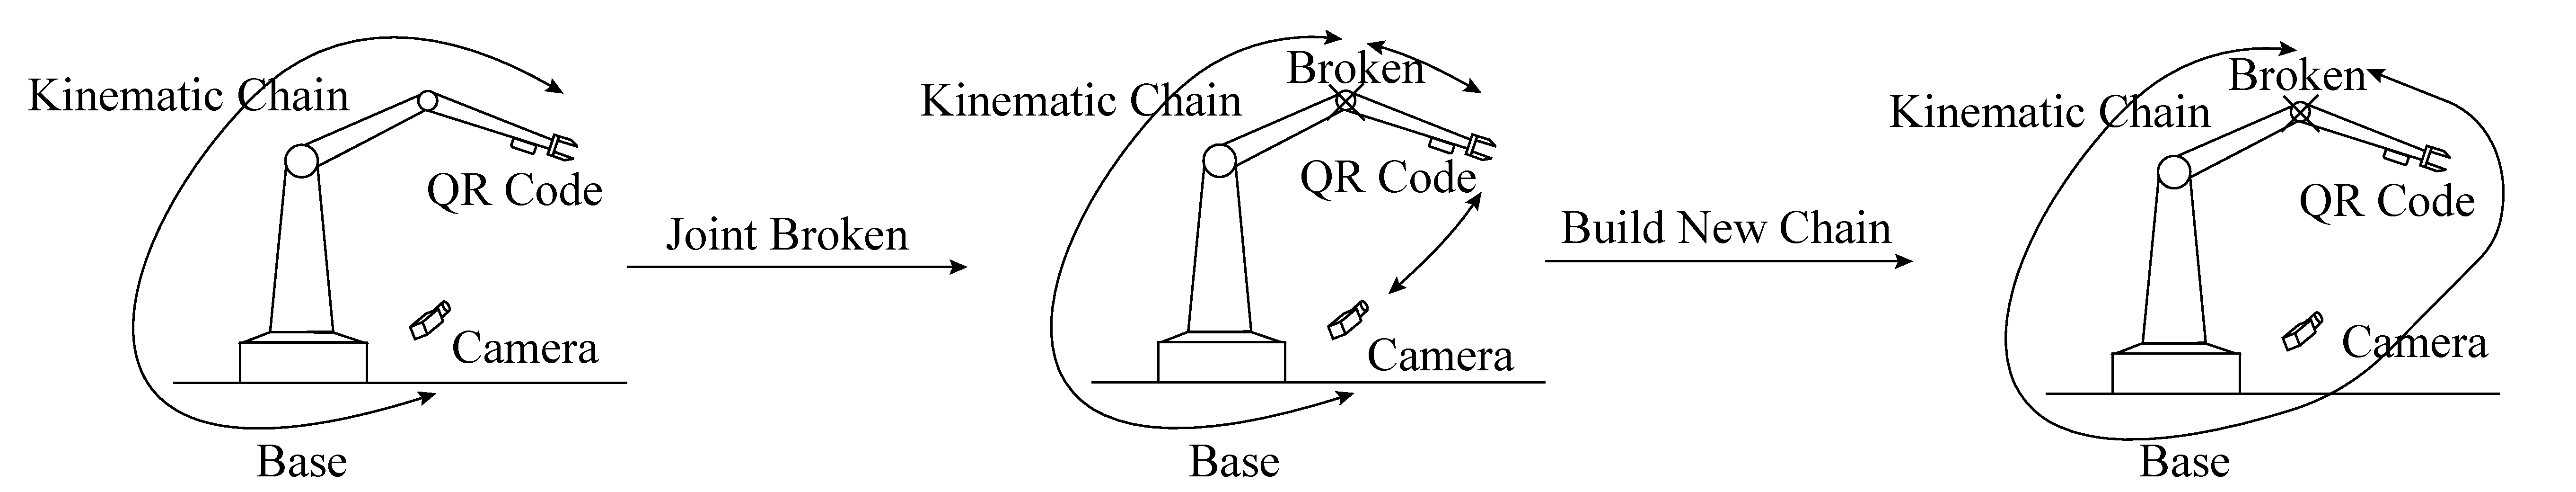
\includegraphics[width=1\textwidth]{img/f1.pdf}
	\caption{ (Left) The original kinematic chain, which is derived from Denavit–-Hartenberg parameters. (Middle) One joint is broken and the kinematic chain is therefore also broken. A QR code on the end-effector is used to estimate the position and orientation of the end effector. (Right) The new  kinematic chain.}
	\label{f1}
\end{figure*}

\subsection{Denavit-Hartenberg parameters}
In mechanical engineering, the Denavit–-Hartenberg parameters \cite{denavit-1955a}(also called DH parameters) are the four parameters associated with a particular convention for attaching reference frames to the links of a spatial kinematic chain, or robot manipulator.
The Kinova $\text{Jaco}^2$ robot arm's DH parameters are shown in Table \ref{dh_parameters}.
%\begin{center}
\begin{table}[!t]
	\centering 
	\caption{}
	\begin{tabular}{ccccc}
		\toprule
		\multicolumn{5}{c}{Kinova $\text{Jaco}^2$ classic DH parameters}\\ 
		\midrule
		\textbf{i}&\textbf{alpha(i-1)}&\textbf{a(i-1)}&\textbf{di}& \textbf{theta1}\\
		\midrule
		\textbf{1}&${\pi}/{2}$&0&0.2755&q1\\
		\midrule
		\textbf{2}&$\pi$&0.4100&0&q2\\
		\midrule
		\textbf{3}&${\pi}/{2}$&0&0.0098&q3\\
		\midrule
		\textbf{4}&${\pi}/{3}$&0&- 0.2501&q4\\
		\midrule
		\textbf{5}&${\pi}/{3}$&0&-0.0856&q5\\
		\midrule
		\textbf{6}&$\pi$&0&-0.2028&q6\\
		\bottomrule
	\end{tabular}
	\label{dh_parameters}
\end{table}
%\end{center}

%\subsection{Apriltag2}
%Subsection text here.

\subsection{Transformation Matrix}
The transformation matrix from coordinate system A to coordinate system B has the following form:

\begin{equation}
\prescript{B}{A}T = 
\left[
\begin{matrix}
R  & t  \\
0 & 1
\end{matrix}
\right] 
\label{TransMat}
\end{equation}

Where $t$ is the translation vector and $R$ is the rotation matrix. The form of $t$ is shown as follows:

\begin{equation}
t =  \left[
\begin{array}{ccc}
x\\
y \\
z
\end{array}
\right] 
\end{equation}

There are three forms of rotation matrix $R$ according to the rotary axis:

\begin{equation}
R_X(\alpha) = 
\left[
\begin{matrix}
1 & 0 & 0 \\
0 & \cos\alpha & -\sin\alpha \\
0 & \sin\alpha & \cos\alpha
\end{matrix}
\right] 
\label{rotation:x}
\end{equation}

\begin{equation}
R_Y(\alpha) = 
\left[
\begin{matrix}
\cos\alpha & 0 & \sin\alpha \\
0 & 1 & 0 \\
-\sin\alpha & 0 & \cos\alpha
\end{matrix}
\right] 
\label{rotation:y}
\end{equation}

\begin{equation}
R_Y(\alpha) = 
\left[
\begin{matrix}
\cos\alpha & -\sin\alpha & 0 \\
\sin\alpha & \cos\alpha & 0 \\
0 & 0 & 1
\end{matrix}
\right] 
\label{rotation:z}
\end{equation}



\subsection{Calculating the joint angle}

Inverse kinematics (IK) makes use of the kinematics equations to determine the joint parameters that provide a desired position for each of the robot's end-effectors.
%The movement of a kinematic chain is modeled by the kinematics equations of the chain. These equations define the configuration of the chain in terms of its joint parameters. 
After setting up a desired position of the end-effectors, we can use the IK algorithm to calculate the joint parameters and send these joint parameters to the motor. However, there is a problem that if the motor and the encoder break, the end-effectors can not achieve the desired point. Usually when an industrial manipulator finds itself in this situation, the broken joint will be immovable due to the low back-drivability. Since the encoder also breaks, that means we don't know the angle of the constrained joint. To make the manipulator adapt from the broken joint, we propose a QR code-based method to calibrate the constrained angle.  

Firstly, we install a web camera near the robot arm's base, and use the hand-eye calibration to calibrate the relative position between robot and camera.

Apriltag2 \cite{wang2016iros} is the QR code we decided to adopt and it is pretty efficient and robust, allowing us to have the exact coordinates of this QR code in the camera coordinate system. Utilizing this feature, we put the QR code on the end-effector so that once the camera sees the QR code it obtains its pose information. Standing from the perspective of DH parameters, we can regard this feature as a virtual link of the manipulator. 

When one of the joints suffers from position failure \cite{maciejewski1990fault,paredis1994kinematic,roberts1996local}, the previous kinematic chain breaks and we can use this virtual link to build a new one. We can predefine several robot arm attitudes to make sure the QR code can be seen and the virtual link can be obtained.

%\begin{figure*}[htpb!]
%  \centering
%  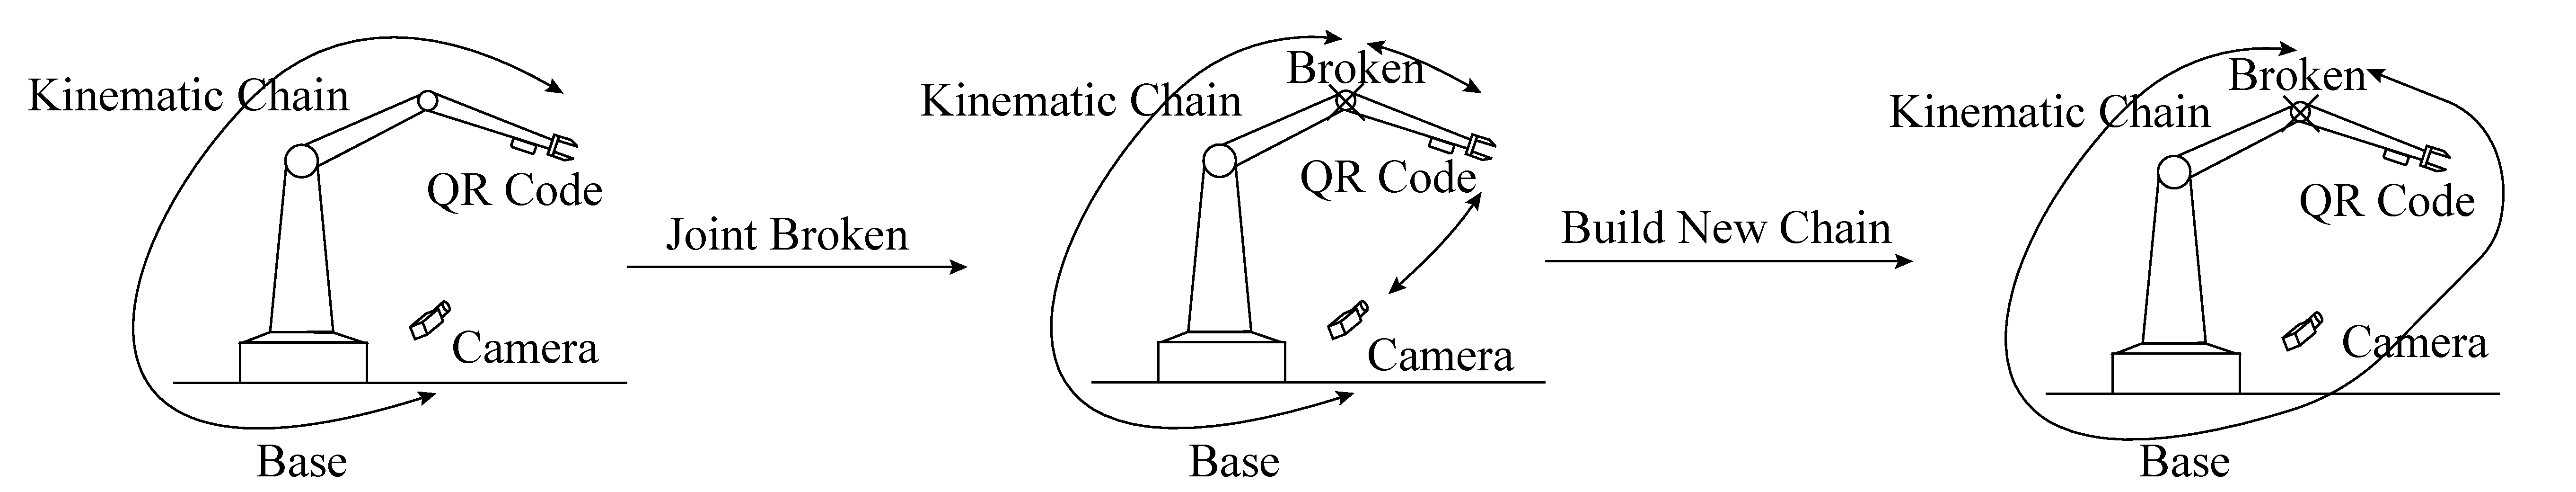
\includegraphics[width=1\textwidth]{img/f1.pdf}
%  \caption{(Left) The original kinematic chain, which is derived from Denavit–-Hartenberg parameters. (Middle) One joint is broken and the kinematic chain is therefore also broken. A QR code on the end-effector is used to estimate the position and orientation of the end effector. (Right) The new  kinematic chain.}
%\label{f1}
%\end{figure*}

A schematic of how our algorithm works can be found in Fig. \ref{f1}. Initially, as we have a manipulator with intact joints the transformation matrix $\prescript{4}{5}{\mathbf{T}}$ is known \emph{a priori}. Assuming, for example, that joint 5 is broken, we will have to build a new chain using the links between base, camera and QR code to build the new transformation matrix $\prescript{4}{5}{\mathbf{T^{'}}}$, using equation \ref{chain:new}. In the equation, the subscript B means base, C means camera, QR means QR code, and E means end-effector.

%\begin{equation}
%\left[ {T} \right] = 
%\left[ {Z_1} \right]
%\left[ {X_1} \right]
%\left[ {Z_2} \right]
%\left[ {X_2} \right]
%\cdots
%\left[ {Z_6} \right]
%\left[ {X_6} \right]
%\end{equation}
%\begin{equation}
%	\prescript{E}{B}{\mathbf{T}} = 	
%	\prescript{E}{6}{\mathbf{T}}
%	\prescript{6}{5}{\mathbf{T}}
%	\prescript{5}{4}{\mathbf{T}}
%	\prescript{4}{3}{\mathbf{T}}
%	\prescript{3}{2}{\mathbf{T}}
%	\prescript{2}{B}{\mathbf{T}}
%\end{equation}

\begin{equation}
\prescript{4}{5}{\mathbf{T^{'}}} = 	
\prescript{4}{3}{\mathbf{T}}
\prescript{3}{2}{\mathbf{T}}
\prescript{2}{B}{\mathbf{T}}
\prescript{B}{C}{\mathbf{T}}
\prescript{C}{QR}{\mathbf{T}}
\prescript{QR}{E}{\mathbf{T}}
\prescript{E}{5}{\mathbf{T}}
\label{chain:new}
\end{equation}


%\begin{equation}
%\begin{split}
% \left[ {T} \right] = 
%&\left[ {Z_3} \right]
%\left[ {X_3} \right]
%\left[ {Z_2} \right]
%\left[ {X_2} \right]
%\left[ Z_{base} \right]
%\left[ X_{base} \right] \\
%& \left[ Z_{camera} \right]
%\left[ C_{camera} \right]
%\left[ Z_{QR} \right]
%\left[ X_{QR} \right]
%\left[ {Z_6} \right]
%\left[ {C_6} \right]\\
%&\left[ {Z_5} \right]
%\left[ {C_5} \right]
%\left[ {Z_4} \right]
%\left[ {C_4} \right]
%\end{split}
%\label{chain:new}
%\end{equation}


At the initial position with our intact manipulator we record $\prescript{4}{5}{\mathbf{T}}$ as a reference matrix. Under the assumption that we know which joint is broken (easily verifiable by a mismatch between control outputs and encoder inputs), we create another transformation matrix $\prescript{4}{5}{\mathbf{T}}^{'}$, using a constrained joint 5 as an example. The difference between $\prescript{4}{5}{\mathbf{T}}$ and $\prescript{4}{5}{\mathbf{T}}^{'}$ lies in the rotation matrix, and the relative position between these two coordinate systems is shown in Fig. \ref{f2}. 
Thus, we can obtain the $\cos\theta$ from the two rotation matrices, and consequently obtain $\theta$ from $\cos\theta$. 

\begin{figure}[t]
	\centering
	\includegraphics[width=0.45\textwidth,height=0.29\textwidth ]{img/f2.pdf}
	\caption{The relative position between  initial  coordinate systems and constrained case coordinate systems. }
	\label{f2}
\end{figure}

\subsection{The adaptive algorithm}

We use a variant of the Newton-Raphson method to solve the inverse kinematic problem of our manipulator. We should find the corresponding joint angles for every single joint, and the Newton-Raphson method enables us to find the root in an iterative process, given a specific x, y, z position. In our problem we need to find the right angles to minimize the difference between the current state position of the end effector of our manipulator and the target position.

Firstly we need to build nonlinear equations: 
\begin{equation}
\begin{cases}
F(\theta) = 0\\
F(\theta) = (f_1,f_2,\dots,f_{12})^T\\
\theta = (\theta_1, \theta_2, \theta_3, \theta_4, \theta_5, \theta_6)^T
\end{cases}
\end{equation}

Each element $f_i$ of $F(\theta)$ is derived by the following way: given the aim homogeneous transformation matrix $\mathbf{T_{aim}}$ of the hand coordinate system to the base coordinate system, 
$\mathbf{T_{aim}}=\mathbf{T_{6}}\mathbf{T_{5}}\mathbf{T_{4}}\mathbf{T_{3}}\mathbf{T_{2}}\mathbf{T_{1}}$,
and for each iteration, we can find a current state homogeneous transformation matrix 
$\mathbf{T_\theta}$,  $\mathbf{T_\theta} = 
\mathbf{T_{\theta_6}}\mathbf{T_{\theta_5}}\mathbf{T_{\theta_4}}\mathbf{T_{\theta_3}}\mathbf{T_{\theta_2}}\mathbf{T_{\theta_1}}$.
The two transformation matrices are both $4 \times 4$, but we just use the upper $3 \times 4$ elements ($\mathbf{T_{11}}$,$\mathbf{T_{12}}$,$\mathbf{T_{13}}$,$\mathbf{T_{14}}$,$\mathbf{T_{21}}$,$\mathbf{T_{22}}$,$\mathbf{T_{23}}$,$\mathbf{T_{24}}$,$\mathbf{T_{31}}$,$\mathbf{T_{32}}$,$\mathbf{T_{33}}$,$\mathbf{T_{34}}$), as the remaining four elements never change. We can subscribe all 12 corresponding entries from the $\mathbf{T_\theta}$ and $\mathbf{T_{aim}}$, one by one, to find $f_i, i=1,2,3 \dots 11,12$. 


Then we can obtain the partial derivatives on $(\theta_1,\theta_2,\theta_3,\theta_4,\theta_5,\theta_6)$
from $F(\theta)$ as the Jacobian matrix $J$, which is $12 \times 6$, and we can find the left inverse of $J$ by $(J^TJ)^{-1}J^T$ as the pseudo inverse J+. Lastly, we use the iteration in the Newton-Raphson algorithm to obtain $\theta^{i+1}$. This workflow is demonstrated in Fig. \ref{f8}.

As we have already calibrated the constrained angle, we update the angles at the end of each iteration and set $\theta^{i}_j = \theta_{calibrated}$, under the assumption that the $j$th joint is broken. Our iteration continues until the difference between $\theta^{i+1}$ and $\theta^{i}$ is below $1e^{-6}$ , and then the trajectory is calculated.

\begin{figure}[t!]
	\centering
	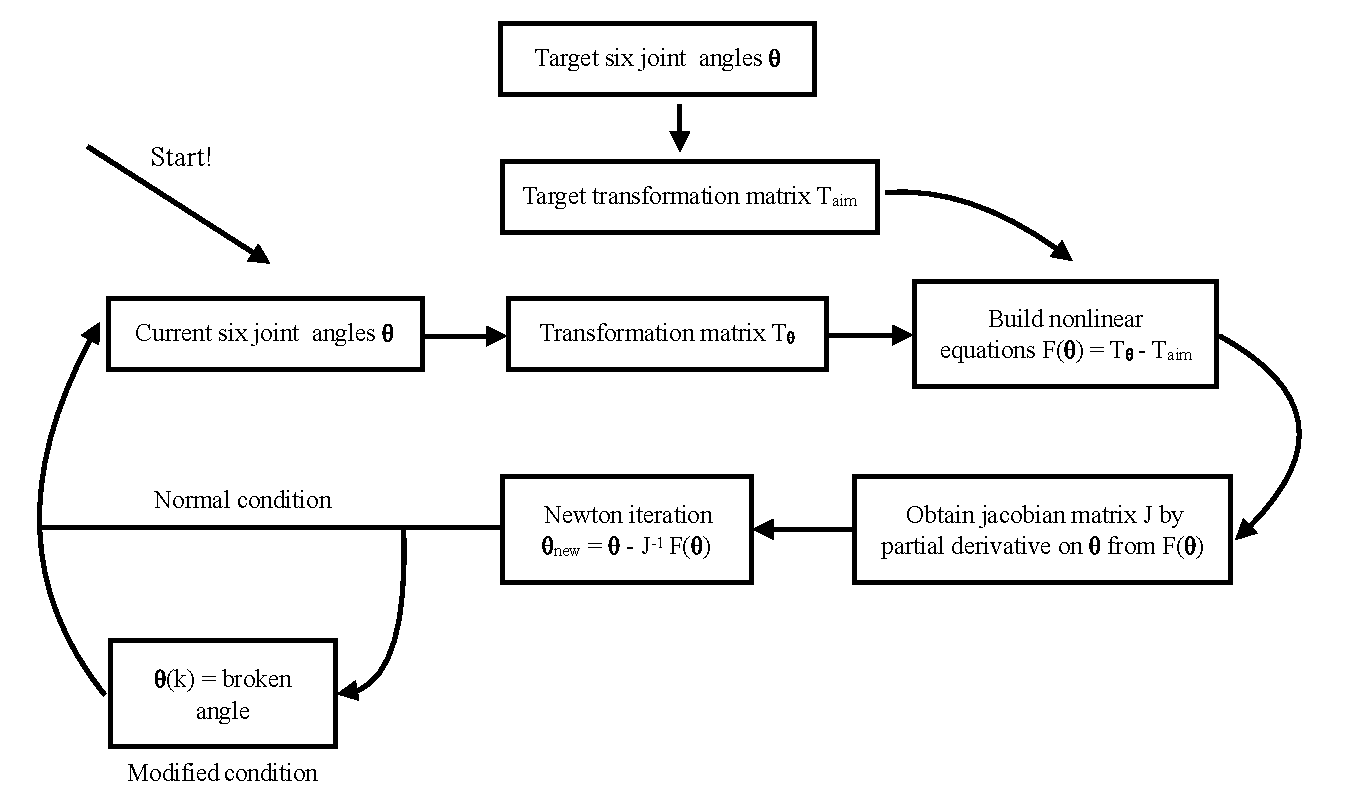
\includegraphics[width=0.47\textwidth]{img/f8.pdf}
	\caption{The pipeline of the variant Newton-Raphson method. It starts from the current position, getting the current joint angles.}
	\label{f8}
\end{figure}

%Since transformation matrix  $\prescript{B}{E}{\mathbf{T}}$ from end-effector coordinate system to the base coordinate system is already known, we can obtain a homogeneous transformation matrix $T_\theta(\theta_1,\theta_2,\theta_3,\theta_4,\theta_5,\theta_6)$ in every iteration.
%Subtract the corresponding elements in the two sets of equations:
%\begin{equation}
%F(\theta) = T_\theta -\prescript{B}{E}{\mathbf{T}}=0
%\label{eq2}
%\end{equation}
%Partial derivative of the variables $(\theta_1,\theta_2,\theta_3,\theta_4,\theta_5,\theta_6)$in the equation \ref{eq2} to obtain the Jacobian matrix$J$
%Then we can calculate the $\theta$ with this formula:
%\begin{equation}
%\theta^{i+1} = \theta^{i} - J^{-1}F(\theta^i)
%\label{form1}
%\end{equation}
%Set $\theta_3$ the value we calibrated in each iteration.

As shown in Fig. \ref{f9}, we register some noise after our calibration with the constrained angle is done, and we decided to take the average angle as our final result. In the figure in question the average angle is $57.6937 \degree$. As the encoder of the Kinova $\text{jaco}^2$ is very accurate, we regard the value shown by the encoder as the ground truth, which is $57.7629 \degree$, yielding in an error of $0.0691 \degree$. Such value, below $0.1 \degree$, is regarded by us as very precise and in par with error values offered by the manufacturer. 

\begin{figure}[t!]
	\centering
	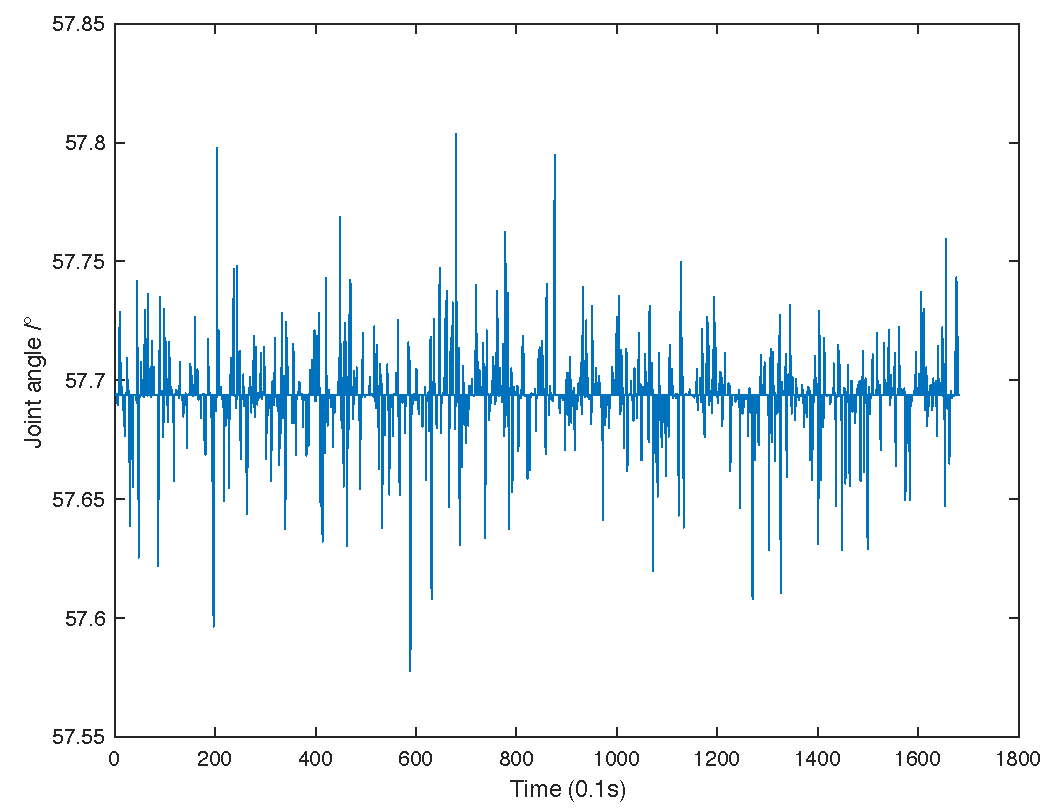
\includegraphics[width=0.47\textwidth,height=0.32\textwidth]{img/f9.pdf}
	\caption{The constrained angle we calibrated. When the camera saw the QR code, we kept calculating the constrained angle every 0.1 seconds. Due to the noise, the value of joint angle is fluctuating. But the general trend is around at $57.6937 \degree$. So we regard it as the constrained angle.}
	\label{f9}
\end{figure}

\subsection{Experimental setting}

We performed our experiments on a Kinova $\text{Jaco}^2$ manipulator. Firstly, we printed an Apriltag2 QR code with a side length of $3 cm$ and placed it on the end-effector. We then 3D printed a camera stand and placed the camera on it, with the relative position between the robot base and this camera being calibrated as proposed in Tsai et al. \cite{tsai1989new}. The transformation matrix $\prescript{QR}{E}{\mathbf{T}}$ between QR code and end-effector can also be obtained through this calibration. 
Kinova $\text{Jaco}^2$ manipulator has a home position and we start our experiment from it. The coordinate of our starting point is $(-0.32,-0.16,0.51)$. In order to verify that our algorithm can work well in the x-axis, y-axis and oblique directions, we chose points A $(0.16,-0.25,0.02)$, B $(-0.16,-0.25,0.02)$ and C $(-0.16,-0.5,0.03)$. In our experiments we mainly adopted paths connecting points A-B, B-C and A-C. A picture of our experimental setup can be found at Fig. \ref{f10}

\begin{figure}[t]
	\centering
	\includegraphics[width=0.47\textwidth,height=0.27\textwidth]{img/f10.jpg}\caption{The environment of our experiment. The QR code is placed on the end-effector, while the camera is at the base. Points A, B and C are used for our experiments.}
	\label{f10}
\end{figure}




% Here you have to talk about the figure "f10". It cannot be in Results, because as I said before, "Results" just talks about the results. "Methods" talks about the methods that you used to achieve the results.
%What robot? What camera? What points? What language? Which OS? Which PC? Which objects to pick up?  Summarising, ALL THE INFORMATION I NEED TO DO THE EXACT SAME EXPERIMENT AND HAVE THE EXACT SAME RESULTS

\section{Results}
\label{section:results}

Once the QR code is seen by the camera, our algorithm instantly starts to calculate the constrained angle, if any problem is detected. We performed series of pick-and place experiments to test our algorithm. As shown in Fig. \ref{f4}, the red line is the trajectory when the robot arm is working normally and the yellow line is the trajectory  when the robot arm's third joint suffers position failure. As one can see, the "defective joint" affects the trajectory of the manipulator and compromises the entire pick-and-place task. Through our adaptive algorithm, shown in blue, the robot arm succeeded with the task. As a pick-and-place activity is a combination of multiple tasks the computational time taken to calculate the new trajectory is close to three minutes, while in simpler operations, such as moving from point A to point B, this time can fall below one minute. Additionally, it is important to note that the constrained joint also affected the start position in a few millimeters.

\begin{figure}[t!]
	\centering 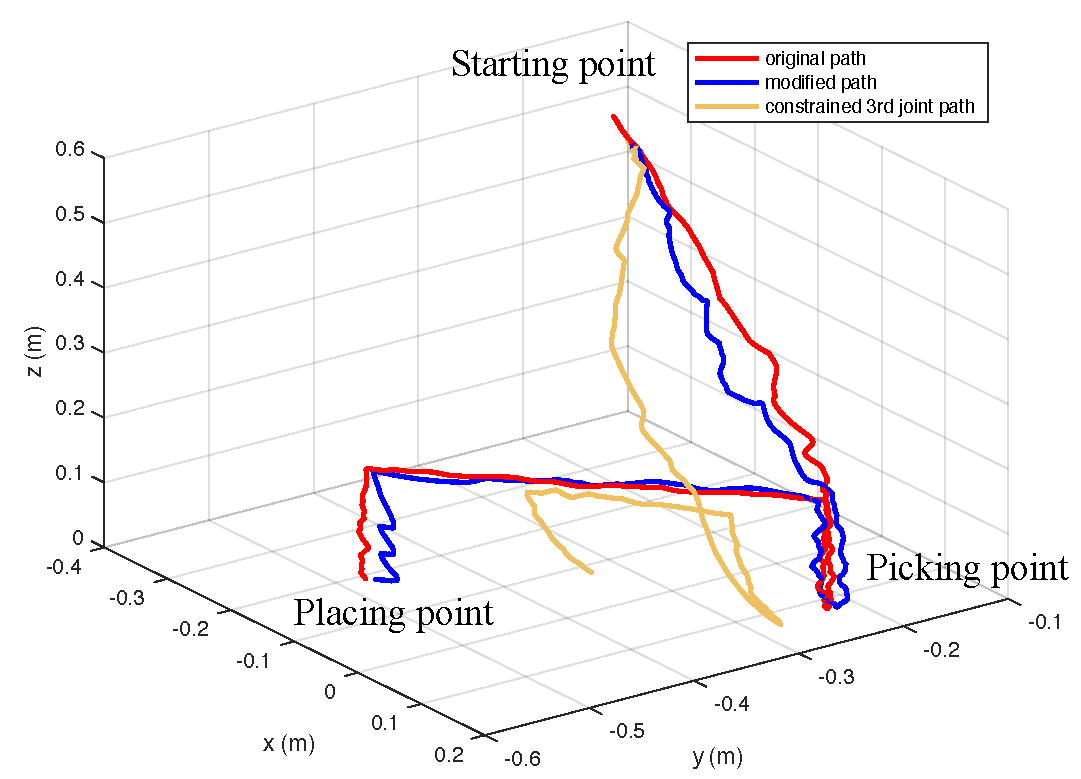
\includegraphics[width=0.47\textwidth]{img/f4.pdf}\caption{Trajectories of three cases. The picking point is set to point A, shown in Fig. \ref{f10}, and the placing point is set to point C. For modified path, we constrain joint 3 at an angle of $50 \degree$. The end-effector first moves directly above the picking point, then closes the gripper and moves up. Then, it moves directly above the placement point, where it moves down to place the object.	}
	\label{f4}
\end{figure}

%To show that the trajectory that calculate every time is a little different but in general, it is still within a fixed range and the planning algorithm can work well instead of accidentally calculating a trajectory.

In order to certify that we can reach the target under multiple conditions, and not by chance in a spurious experiment, we performed seven repeated experiments to move the end-effector from starting point $(-0.32,-0.16,0.51)$ to end point $(0.	20, -0.45, 0.02)$. Our results, in Fig. \ref{f5}, show that although our algorithm predicts different corrective measures along the trajectory, the differences between these trajectories are very small, and our method always converges to the intended final goal in a high repeatability.

\begin{figure}[tb!]
	\centering
	%test.m file
	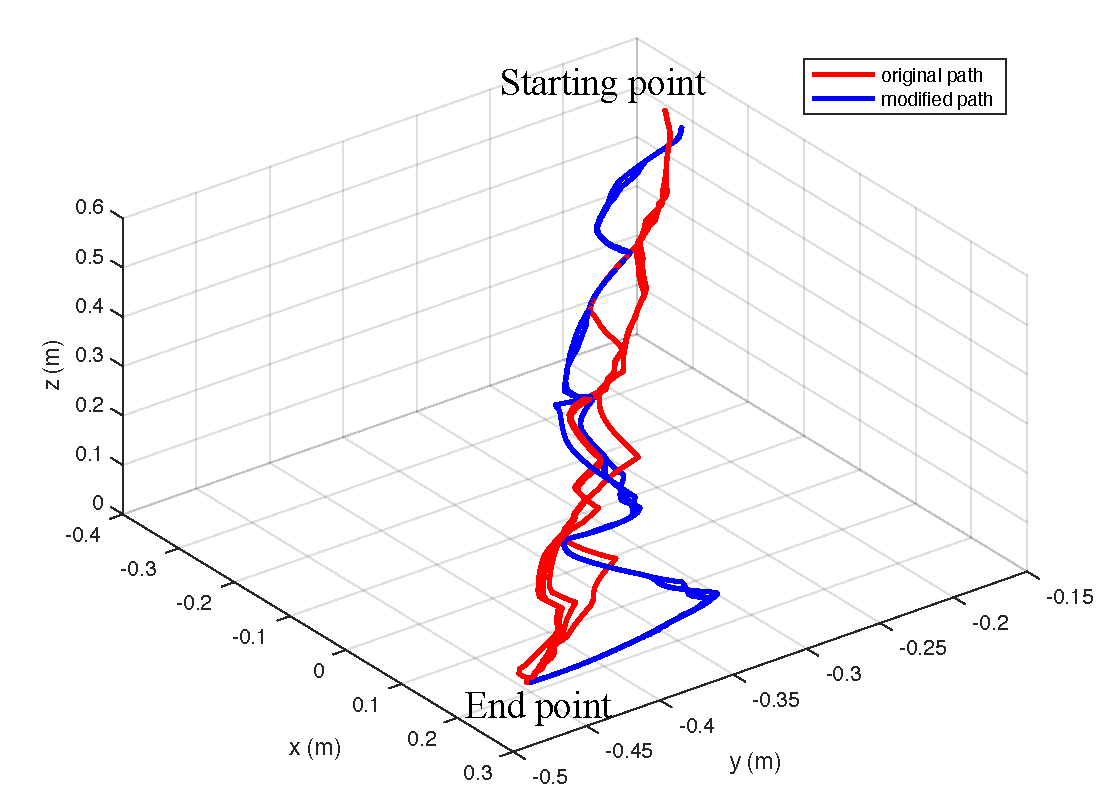
\includegraphics[width=0.47\textwidth]{img/f5.pdf} \caption{The trajectories of the end-effector, from start point to end point, under the original algorithm and our Adaptive algorithm. Each algorithm has seven trajectories, and we constrained joint 3 at an angle of $70 \degree$.  The seven trajectories of our algorithm are almost coincident. 	}
	\label{f5}
\end{figure}

To better understand the influence of the differences seen in the previous experiment, we evaluated individual joints in the same point-to-point experiment. The Fig. \ref{f6} shows the rotation of six joints under the original algorithm and our Adaptive algorithm. It can be seen that due to the constraint in joint 3 (green) the rotations of the other joints had to adapt considerably. 

% Why is the experiment slow (I mean, the manipulator is moving so slowly and taking 25 seconds to reach the target, as seen in Fig. 8)


\begin{figure}[tb!] \centering 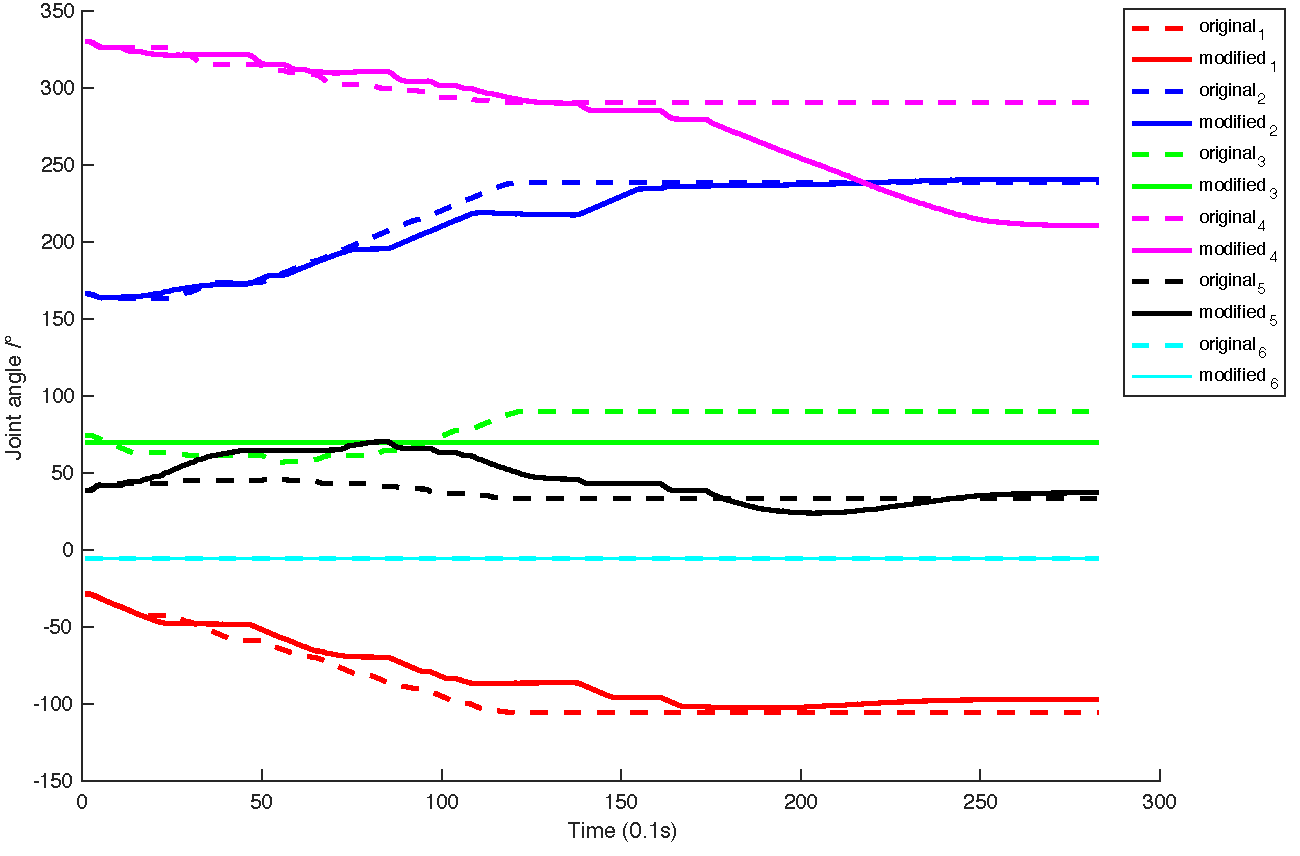
\includegraphics[width=0.47\textwidth]{img/f6.pdf} \caption{ The changes in six joints, from start point to end point, under the original algorithm and our Adaptive algorithm. We constrained joint 3 at an angle of $70 \degree$. The rotation of joints are different under the two algorithms, but eventually they reach the same target point.	}
	\label{f6}
\end{figure}

As changes in joint angles of a manipulator might also affect negatively the final orientation of the end-effector, which could prevent the manipulator from ultimately performing the action that it was intended to do, we also compared the roll, pitch and yaw of the end-effector under these two algorithms. As can be seen from Fig. \ref{f7}, when the joint is constrained the end-effector will deviate from the target and the grasp will fail. At the same time, although our adaptive algorithm successfully captured the target object, the orientation of the end-effector changed.

\begin{figure}[tb!]
	\centering \includegraphics[width=0.47\textwidth]{img/f7.pdf} \caption{The change in roll, pitch, yaw under two algorithms. Comparing the original, modified and constrained paths we can see the changes in orientation.}
	\label{f7}
\end{figure}

Finally, we decided to verify the extent to which the manipulator can still maintain function after a range of malfunctions on different joints. We chose different angle values to constrain our joints at, and focused on joints 3, 4 and 5. We chose these joints based on the work from \cite{nakamura1987task} . According to this work, DOFs from a manipulator can be divided into two groups: Major DOFs (MDOFs) which are critical in performing a task, and Secondary DOFs, which are less important and replaceable to a certain degree. If a SDOF suffers position failure, the manipulator has a higher probability to modify itself and reach the goal.

\begin{table}[!hb]
	\centering
	\caption{The robustness of our algorithm with different constrained angle in different joints }\label{tab:aStrangeTable}%添加标题 设置标签
	\begin{threeparttable}
		\begin{tabular}{cccc}
			\toprule
			\textbf{Angle}& \textbf{Joint 3}& \textbf{Joint 4}& \textbf{Joint 5}\\
			\midrule
			\textbf{$30\degree $}& FAIL& SUCCESS&SUCCESS\\
			\textbf{$50\degree $}& SUCCESS& SUCCESS&SUCCESS\\
			\textbf{$70\degree $}& SUCCESS& SUCCESS&SUCCESS\\
			\textbf{$90\degree $}& FAIL& SUCCESS&SUCCESS\\
			\textbf{$110\degree $}& FAIL& SUCCESS&FAIL\\
			\textbf{$130\degree $}& FAIL& SUCCESS&FAIL\\
			\textbf{$150\degree $}& FAIL& SUCCESS&FAIL\\
			\bottomrule
		\end{tabular}
		\begin{tablenotes}
			\footnotesize
			\item[1] SUCCESS means the end-effector can reach the target point.
			\item[2] FAIL means the end-effector can not reach the target point.
		\end{tablenotes}
	\end{threeparttable}
\end{table}

As the Table \ref{tab:aStrangeTable} shows, joint 3 is a MDOF, so the operation range of this joint in the eventuality of a malfunction is limited (between $50\degree$ and $70\degree$). Since joint 4 is a secondary DOF (SDOFs)\cite{nakamura1987task} , the tolerable range is very large. However, even though joint 5 is a SDOF, due to the long length of the link the tolerable range is of $60\degree $. We assumed that joint 1 and 2 are MDOFs, and failure in those joints would immediately constrain the positioning of the end-effector. Joint 6, on the other hand, although redundant when positioning is considered, is very important for the orientation of the end-effector. A video with our experiments can be found here: https://youtu.be/WaoXPJuKEvs .

%What about 6? What about 1 and 2?

\section{Discussion}
\label{section:discussion}

\subsection{Influence on orientation}

With regards to the orientation after the malfunction, the results from Fig. \ref{f7} and Table \ref{tab:aStrangeTable} lead us to believe that our algorithm can be used as a useful back-up plan to be implemented while a definitive solution (or the scheduled maintenance) takes place. As objects are approached from above in pick-and-place tasks, common in industrial assembly lines, the presence of a $180\degree$ dome of grasping affordances might not be a reality, and this can be a limiting factor for the success of our algorithm. However, previous authors, from either model-based \cite{7832455} or learning-based \cite{goel2005analyzing} \cite{cully2015robots} \ref{f9} approaches were also hindered by similar problems, and we believe that the ideal solution would go beyond adaptation, by allowing robots to fix their motors/sensors. 

Malfunctions are not all the same: When a motor malfunction takes place instead of a sensor malfunction, there is no need for a self-calibration. The works \cite{goel2005analyzing} and \cite{7832455} assume knowledge of all joint angles, and in this case the problem can be bluntly written as a reduction to $N-1$ DOF, with a frozen link. Sensors can break, cables can be disconnected, or just suffer from unknown noise sources, and when the closed-loop motor control is compromised our self-calibration combined with the adaptation algorithm is vital for the task continuity. The precision of our algorithm in predicting the angle of the constrained joint, shown in Fig. \ref{f9}, demonstrates that we can reliably overcome the absence of a sensor on a joint by adding vision to our system.

\subsection{Try not. Do, or do not}

Solutions can range from model-based to learning-based approaches, but from the assumption that robot arms are manufactured by engineering companies we can easily conclude that a prior knowledge of that chosen morphology already exists. Ignorance over such prior, starting from a \emph{tabula rasa}, will slow down convergence as previously demonstrated with a five dimensional real-world-based problem taking 72 hours to converge \cite{rosendo2017trade}. 

Simulation-based learning, on the other hand, could drastically reduce this time, but these are often used as benchmarks for robots learning new tasks, not old ones. As a computer simulation requires a model to simulate, the presence of such model can speed up iterations, but if the manipulator model is accurate (intact joints and links) the computational time to reach a Cartesian coordinate through iterations would be superior to the same task with Inverse Kinematics.

Simulations combined with real-world, as shown by \cite{cully2015robots} and \cite{chatzilygeroudis2017black}, can be very powerful methods to account for malfunctions. These works show that a simulation can take place in an inaccurate model to create a coarse prior knowledge, while data-efficient real-world iterations can minimise the iteration time and guarantee transferability to the real-world. Such methods can account for motor and sensor malfunctions, and even go beyond, also assuming broken links. However, one major drawback from these methods lie in the computational time: while our method takes a maximum of three minutes for a multi-point pick-and-place and less than one minute for single point-to-point tasks, learning algorithms are notoriously intensive on their approach to data. As an example, the 15 seconds of iteration time from \cite{chatzilygeroudis2017black} in a cart-pole balancing problem required 25 minutes to compute 8 learning episodes.

In addition to the time taken to converge to a solution, prior-based physical learning (or also called Grey-box methods, as they have Black-box and White-box elements \cite{kroll2000grey}) requires trials to find a solution (the higher the required precision the more trials). From an industrial perspective, having to produce defective products to reach a commercialisable final product is unacceptable. Beyond being easily implemented with one inexpensive camera, guaranteeing a high precision of the end-effector positioning, and taking a few minutes to calculate a new trajectory, in our proposed method "there is no try".

\subsection{Limitations}

The position error that we present in this work can still be considered too big for specific industrial applications, and it is an accumulation of the hand-eye calibration error, camera calibration error and QR code error. Still, since we only use one inexpensive camera with one ink-jet printer-printed QR code there is still room for improvement in the final precision, by combining higher resolution cameras with multiple QR codes and go below the millimetric scale. 

From Fig. \ref{f5} we could see that our proposed trajectory suffers minor deviations while following their path, and we believe that such differences arise from the truncation error on sensor sampling and motor commands. It is important to observe that the original path planning from Kinova $\text{Jaco}^2$ manipulator also showed a similar behavior, albeit at a smaller scale. Although the uncertainty associated with the new path might represent a problem for industrial settings with highly-constrained operation spaces, this possible problem can be easily prevented with the addition of via points to the original trajectory. Additionally, our Adaptive algorithm is only meant as a stop-gap procedure until a formal repair can be implemented to the manipulator during the scheduled maintenance.

The time to calculate a new trajectory, which can reach three minutes of computation, can still be further improved. As we are currently using Python, a high-level scripting language, the execution is slow. We are currently rewriting our algorithm in C language to maximise performance. Additionally, we also plan on modifying the Jacobian matrix, shown in Fig. \ref{f8} in a iterative process \cite{chen2003optimal}, or multi-thread (CPU cores or FPGA) the calculation of the IK to increase the speed.

One of the current shortcomings for our calibration method is when the QR code is not within the visible range of the camera (due to the angle at which the malfunction happened), and the virtual link cannot be established. In such cases the manipulator needs to rotate the remaining normal joints of the robot arm to let the QR code enter the camera's field of view. Alternatively, we can increase the number of QR codes to reduce the probability of such eventuality happening.


\section{Conclusion}
\label{section:conclusion}

% Figure \ref{f9} shows that our scheme can calibrate the constrained angle successfully and the error is less than $0.1\degree$. 
% For a 6DOFs manipulator, our adaptive algorithm works well when redundant joint is damage. 
% But for the MDOFs like the joint 1, this adaptive algorithm cannot compensate for the defects.

We proposed a method capable of overcoming position failure and sensor failure on an industrial manipulator, with a high accuracy, quick computational time and inexpensive. Since our method only uses a web camera and a printed QR code per manipulator, the cost of upscaling this method to allow every manipulator within a factory to adapt to malfunctions is negligible. Also, as our method utilizes known models of commercially available robots it can be easily deployed to a plethora of robot arms and snake robots.

In the future, we believe that our method will be very useful for fully autonomous factories and on search-and-rescue snake robots. The probability of failures increase in systems with a large number of robots and of joints, and our method permits these systems to keep going without compromising on precision. 
Compared with the costly portable photogrammetry system (e.g., the MaxSHOT 3D\cite{filion2018robot} is more than $\$100,000$ and a Faro laser tracker is about $\$50,000)$ and the camera based photogrammetric approach which can only determine the pose of the robot end-effector, our method is inexpensive and can compute almost every joint which is broken. It works well on our Kinova $\text{Jaco}^2$ robot arm. And it can be easily implemented at an industrial robot arm by the factory workers, which shows the width range of commerce scenarios.
In the future we will extend this work to allow the simultaneous calibration of two or more constrained joints, and also test similar techniques to bring precision to soft robotics.

\subsection{Abbreviations and Acronyms}
Define abbreviations and acronyms the first time they are used in the text, 
even after they have already been defined in the abstract. Abbreviations 
such as IEEE, SI, ac, and dc do not have to be defined. Abbreviations that 
incorporate periods should not have spaces: write ``C.N.R.S.,'' not ``C. N. 
R. S.'' Do not use abbreviations in the title unless they are unavoidable 
(for example, ``IEEE'' in the title of this article).

\subsection{Other Recommendations}
Use one space after periods and colons. Hyphenate complex modifiers: 
``zero-field-cooled magnetization.'' Avoid dangling participles, such as, 
``Using \eqref{eq}, the potential was calculated.'' [It is not clear who or what 
used \eqref{eq}.] Write instead, ``The potential was calculated by using \eqref{eq},'' or 
``Using \eqref{eq}, we calculated the potential.''

Use a zero before decimal points: ``0.25,'' not ``.25.'' Use 
``cm$^{3}$,'' not ``cc.'' Indicate sample dimensions as ``0.1 cm 
$\times $ 0.2 cm,'' not ``0.1 $\times $ 0.2 cm$^{2}$.'' The 
abbreviation for ``seconds'' is ``s,'' not ``sec.'' Use 
``Wb/m$^{2}$'' or ``webers per square meter,'' not 
``webers/m$^{2}$.'' When expressing a range of values, write ``7 to 
9'' or ``7--9,'' not ``7$\sim $9.''

A parenthetical statement at the end of a sentence is punctuated outside of 
the closing parenthesis (like this). (A parenthetical sentence is punctuated 
within the parentheses.) In American English, periods and commas are within 
quotation marks, like ``this period.'' Other punctuation is ``outside''! 
Avoid contractions; for example, write ``do not'' instead of ``don't.'' The 
serial comma is preferred: ``A, B, and C'' instead of ``A, B and C.''

If you wish, you may write in the first person singular or plural and use 
the active voice (``I observed that $\ldots$'' or ``We observed that $\ldots$'' 
instead of ``It was observed that $\ldots$''). Remember to check spelling. If 
your native language is not English, please get a native English-speaking 
colleague to carefully proofread your paper.

Try not to use too many typefaces in the same article. You're writing
scholarly papers, not ransom notes. Also please remember that MathJax
can't handle really weird typefaces.

\subsection{Equations}
Number equations consecutively with equation numbers in parentheses flush 
with the right margin, as in \eqref{eq}. To make your equations more 
compact, you may use the solidus (~/~), the exp function, or appropriate 
exponents. Use parentheses to avoid ambiguities in denominators. Punctuate 
equations when they are part of a sentence, as in
\begin{equation}E=mc^2.\label{eq}\end{equation}

Be sure that the symbols in your equation have been defined before the 
equation appears or immediately following. Italicize symbols ($T$ might refer 
to temperature, but T is the unit tesla). Refer to ``\eqref{eq},'' not ``Eq. \eqref{eq}'' 
or ``equation \eqref{eq},'' except at the beginning of a sentence: ``Equation \eqref{eq} 
is $\ldots$ .''

\subsection{\LaTeX-Specific Advice}

Please use ``soft'' (e.g., \verb|\eqref{Eq}|) cross references instead
of ``hard'' references (e.g., \verb|(1)|). That will make it possible
to combine sections, add equations, or change the order of figures or
citations without having to go through the file line by line.

Please don't use the \verb|{eqnarray}| equation environment. Use
\verb|{align}| or \verb|{IEEEeqnarray}| instead. The \verb|{eqnarray}|
environment leaves unsightly spaces around relation symbols.

Please note that the \verb|{subequations}| environment in {\LaTeX}
will increment the main equation counter even when there are no
equation numbers displayed. If you forget that, you might write an
article in which the equation numbers skip from (17) to (20), causing
the copy editors to wonder if you've discovered a new method of
counting.

{\BibTeX} does not work by magic. It doesn't get the bibliographic
data from thin air but from .bib files. If you use {\BibTeX} to produce a
bibliography you must send the .bib files. 

{\LaTeX} can't read your mind. If you assign the same label to a
subsubsection and a table, you might find that Table I has been cross
referenced as Table IV-B3. 

{\LaTeX} does not have precognitive abilities. If you put a
\verb|\label| command before the command that updates the counter it's
supposed to be using, the label will pick up the last counter to be
cross referenced instead. In particular, a \verb|\label| command
should not go before the caption of a figure or a table.

Do not use \verb|\nonumber| inside the \verb|{array}| environment. It
will not stop equation numbers inside \verb|{array}| (there won't be
any anyway) and it might stop a wanted equation number in the
surrounding equation.

\section{Units}
Use either SI (MKS) or CGS as primary units. (SI units are strongly 
encouraged.) English units may be used as secondary units (in parentheses). 
This applies to papers in data storage. For example, write ``15 
Gb/cm$^{2}$ (100 Gb/in$^{2})$.'' An exception is when 
English units are used as identifiers in trade, such as ``3\textonehalf-in 
disk drive.'' Avoid combining SI and CGS units, such as current in amperes 
and magnetic field in oersteds. This often leads to confusion because 
equations do not balance dimensionally. If you must use mixed units, clearly 
state the units for each quantity in an equation.

The SI unit for magnetic field strength $H$ is A/m. However, if you wish to use 
units of T, either refer to magnetic flux density $B$ or magnetic field 
strength symbolized as $\mu _{0}H$. Use the center dot to separate 
compound units, e.g., ``A$\cdot $m$^{2}$.''

\section{Some Common Mistakes}
The word ``data'' is plural, not singular. The subscript for the 
permeability of vacuum $\mu _{0}$ is zero, not a lowercase letter 
``o.'' The term for residual magnetization is ``remanence''; the adjective 
is ``remanent''; do not write ``remnance'' or ``remnant.'' Use the word 
``micrometer'' instead of ``micron.'' A graph within a graph is an 
``inset,'' not an ``insert.'' The word ``alternatively'' is preferred to the 
word ``alternately'' (unless you really mean something that alternates). Use 
the word ``whereas'' instead of ``while'' (unless you are referring to 
simultaneous events). Do not use the word ``essentially'' to mean 
``approximately'' or ``effectively.'' Do not use the word ``issue'' as a 
euphemism for ``problem.'' When compositions are not specified, separate 
chemical symbols by en-dashes; for example, ``NiMn'' indicates the 
intermetallic compound Ni$_{0.5}$Mn$_{0.5}$ whereas 
``Ni--Mn'' indicates an alloy of some composition 
Ni$_{x}$Mn$_{1-x}$.

\Figure[t!](topskip=0pt, botskip=0pt, midskip=0pt){fig1.png}
{Magnetization as a function of applied field.
It is good practice to explain the significance of the figure in the caption.\label{fig1}}

Be aware of the different meanings of the homophones ``affect'' (usually a 
verb) and ``effect'' (usually a noun), ``complement'' and ``compliment,'' 
``discreet'' and ``discrete,'' ``principal'' (e.g., ``principal 
investigator'') and ``principle'' (e.g., ``principle of measurement''). Do 
not confuse ``imply'' and ``infer.'' 

Prefixes such as ``non,'' ``sub,'' ``micro,'' ``multi,'' and ``ultra'' are 
not independent words; they should be joined to the words they modify, 
usually without a hyphen. There is no period after the ``et'' in the Latin 
abbreviation ``\emph{et al.}'' (it is also italicized). The abbreviation ``i.e.,'' means 
``that is,'' and the abbreviation ``e.g.,'' means ``for example'' (these 
abbreviations are not italicized).

A general IEEE styleguide is available at \underline{http://www.ieee.org/}\break\underline{authortools}.

\section{Guidelines for Graphics Preparation and Submission}
\label{sec:guidelines}

\subsection{Types of Graphics}
The following list outlines the different types of graphics published in 
IEEE journals. They are categorized based on their construction, and use of 
color/shades of gray:

\subsubsection{Color/Grayscale figures}
{Figures that are meant to appear in color, or shades of black/gray. Such 
figures may include photographs, illustrations, multicolor graphs, and 
flowcharts.}

\subsubsection{Line Art figures}
{Figures that are composed of only black lines and shapes. These figures 
should have no shades or half-tones of gray, only black and white.}

\subsubsection{Author photos}
{Head and shoulders shots of authors that appear at the end of our papers. }

\subsubsection{Tables}
{Data charts which are typically black and white, but sometimes include 
color.}

\begin{table}
\caption{Units for Magnetic Properties}
\label{table}
\setlength{\tabcolsep}{3pt}
\begin{tabular}{|p{25pt}|p{75pt}|p{115pt}|}
\hline
Symbol& 
Quantity& 
Conversion from Gaussian and \par CGS EMU to SI $^{\mathrm{a}}$ \\
\hline
$\Phi $& 
magnetic flux& 
1 Mx $\to  10^{-8}$ Wb $= 10^{-8}$ V$\cdot $s \\
$B$& 
magnetic flux density, \par magnetic induction& 
1 G $\to  10^{-4}$ T $= 10^{-4}$ Wb/m$^{2}$ \\
$H$& 
magnetic field strength& 
1 Oe $\to  10^{3}/(4\pi )$ A/m \\
$m$& 
magnetic moment& 
1 erg/G $=$ 1 emu \par $\to 10^{-3}$ A$\cdot $m$^{2} = 10^{-3}$ J/T \\
$M$& 
magnetization& 
1 erg/(G$\cdot $cm$^{3}) =$ 1 emu/cm$^{3}$ \par $\to 10^{3}$ A/m \\
4$\pi M$& 
magnetization& 
1 G $\to  10^{3}/(4\pi )$ A/m \\
$\sigma $& 
specific magnetization& 
1 erg/(G$\cdot $g) $=$ 1 emu/g $\to $ 1 A$\cdot $m$^{2}$/kg \\
$j$& 
magnetic dipole \par moment& 
1 erg/G $=$ 1 emu \par $\to 4\pi \times  10^{-10}$ Wb$\cdot $m \\
$J$& 
magnetic polarization& 
1 erg/(G$\cdot $cm$^{3}) =$ 1 emu/cm$^{3}$ \par $\to 4\pi \times  10^{-4}$ T \\
$\chi , \kappa $& 
susceptibility& 
1 $\to  4\pi $ \\
$\chi_{\rho }$& 
mass susceptibility& 
1 cm$^{3}$/g $\to  4\pi \times  10^{-3}$ m$^{3}$/kg \\
$\mu $& 
permeability& 
1 $\to  4\pi \times  10^{-7}$ H/m \par $= 4\pi \times  10^{-7}$ Wb/(A$\cdot $m) \\
$\mu_{r}$& 
relative permeability& 
$\mu \to \mu_{r}$ \\
$w, W$& 
energy density& 
1 erg/cm$^{3} \to  10^{-1}$ J/m$^{3}$ \\
$N, D$& 
demagnetizing factor& 
1 $\to  1/(4\pi )$ \\
\hline
\multicolumn{3}{p{251pt}}{Vertical lines are optional in tables. Statements that serve as captions for 
the entire table do not need footnote letters. }\\
\multicolumn{3}{p{251pt}}{$^{\mathrm{a}}$Gaussian units are the same as cg emu for magnetostatics; Mx 
$=$ maxwell, G $=$ gauss, Oe $=$ oersted; Wb $=$ weber, V $=$ volt, s $=$ 
second, T $=$ tesla, m $=$ meter, A $=$ ampere, J $=$ joule, kg $=$ 
kilogram, H $=$ henry.}
\end{tabular}
\label{tab1}
\end{table}

\subsection{Multipart figures}
Figures compiled of more than one sub-figure presented side-by-side, or 
stacked. If a multipart figure is made up of multiple figure
types (one part is lineart, and another is grayscale or color) the figure 
should meet the stricter guidelines.

\subsection{File Formats For Graphics}\label{formats}
Format and save your graphics using a suitable graphics processing program 
that will allow you to create the images as PostScript (PS), Encapsulated 
PostScript (.EPS), Tagged Image File Format (.TIFF), Portable Document 
Format (.PDF), Portable Network Graphics (.PNG), or Metapost (.MPS), sizes them, and adjusts 
the resolution settings. When 
submitting your final paper, your graphics should all be submitted 
individually in one of these formats along with the manuscript.

\subsection{Sizing of Graphics}
Most charts, graphs, and tables are one column wide (3.5 inches/88 
millimeters/21 picas) or page wide (7.16 inches/181 millimeters/43 
picas). The maximum depth a graphic can be is 8.5 inches (216 millimeters/54
picas). When choosing the depth of a graphic, please allow space for a 
caption. Figures can be sized between column and page widths if the author 
chooses, however it is recommended that figures are not sized less than 
column width unless when necessary. 

There is currently one publication with column measurements that do not 
coincide with those listed above. Proceedings of the IEEE has a column 
measurement of 3.25 inches (82.5 millimeters/19.5 picas). 

The final printed size of author photographs is exactly
1 inch wide by 1.25 inches tall (25.4 millimeters$\,\times\,$31.75 millimeters/6 
picas$\,\times\,$7.5 picas). Author photos printed in editorials measure 1.59 inches 
wide by 2 inches tall (40 millimeters$\,\times\,$50 millimeters/9.5 picas$\,\times\,$12 
picas).

\subsection{Resolution }
The proper resolution of your figures will depend on the type of figure it 
is as defined in the ``Types of Figures'' section. Author photographs, 
color, and grayscale figures should be at least 300dpi. Line art, including 
tables should be a minimum of 600dpi.

\subsection{Vector Art}
In order to preserve the figures' integrity across multiple computer 
platforms, we accept files in the following formats: .EPS/.PDF/.PS. All 
fonts must be embedded or text converted to outlines in order to achieve the 
best-quality results.

\subsection{Color Space}
The term color space refers to the entire sum of colors that can be 
represented within the said medium. For our purposes, the three main color 
spaces are Grayscale, RGB (red/green/blue) and CMYK 
(cyan/magenta/yellow/black). RGB is generally used with on-screen graphics, 
whereas CMYK is used for printing purposes.

All color figures should be generated in RGB or CMYK color space. Grayscale 
images should be submitted in Grayscale color space. Line art may be 
provided in grayscale OR bitmap colorspace. Note that ``bitmap colorspace'' 
and ``bitmap file format'' are not the same thing. When bitmap color space 
is selected, .TIF/.TIFF/.PNG are the recommended file formats.

\subsection{Accepted Fonts Within Figures}
When preparing your graphics IEEE suggests that you use of one of the 
following Open Type fonts: Times New Roman, Helvetica, Arial, Cambria, and 
Symbol. If you are supplying EPS, PS, or PDF files all fonts must be 
embedded. Some fonts may only be native to your operating system; without 
the fonts embedded, parts of the graphic may be distorted or missing.

A safe option when finalizing your figures is to strip out the fonts before 
you save the files, creating ``outline'' type. This converts fonts to 
artwork what will appear uniformly on any screen.

\subsection{Using Labels Within Figures}

\subsubsection{Figure Axis labels }
Figure axis labels are often a source of confusion. Use words rather than 
symbols. As an example, write the quantity ``Magnetization,'' or 
``Magnetization M,'' not just ``M.'' Put units in parentheses. Do not label 
axes only with units. As in Fig. 1, for example, write ``Magnetization 
(A/m)'' or ``Magnetization (A$\cdot$m$^{-1}$),'' not just ``A/m.'' Do not label axes with a ratio of quantities and 
units. For example, write ``Temperature (K),'' not ``Temperature/K.'' 

Multipliers can be especially confusing. Write ``Magnetization (kA/m)'' or 
``Magnetization (10$^{3}$ A/m).'' Do not write ``Magnetization 
(A/m)$\,\times\,$1000'' because the reader would not know whether the top 
axis label in Fig. 1 meant 16000 A/m or 0.016 A/m. Figure labels should be 
legible, approximately 8 to 10 point type.

\subsubsection{Subfigure Labels in Multipart Figures and Tables}
Multipart figures should be combined and labeled before final submission. 
Labels should appear centered below each subfigure in 8 point Times New 
Roman font in the format of (a) (b) (c). 

\subsection{File Naming}
Figures (line artwork or photographs) should be named starting with the 
first 5 letters of the author's last name. The next characters in the 
filename should be the number that represents the sequential 
location of this image in your article. For example, in author 
``Anderson's'' paper, the first three figures would be named ander1.tif, 
ander2.tif, and ander3.ps.

Tables should contain only the body of the table (not the caption) and 
should be named similarly to figures, except that `.t' is inserted 
in-between the author's name and the table number. For example, author 
Anderson's first three tables would be named ander.t1.tif, ander.t2.ps, 
ander.t3.eps.

Author photographs should be named using the first five characters of the 
pictured author's last name. For example, four author photographs for a 
paper may be named: oppen.ps, moshc.tif, chen.eps, and duran.pdf.

If two authors or more have the same last name, their first initial(s) can 
be substituted for the fifth, fourth, third$\ldots$ letters of their surname 
until the degree where there is differentiation. For example, two authors 
Michael and Monica Oppenheimer's photos would be named oppmi.tif, and 
oppmo.eps.

\subsection{Referencing a Figure or Table Within Your Paper}
When referencing your figures and tables within your paper, use the 
abbreviation ``Fig.'' even at the beginning of a sentence. Do not abbreviate 
``Table.'' Tables should be numbered with Roman Numerals.

\subsection{Checking Your Figures: The IEEE Graphics Analyzer}
The IEEE Graphics Analyzer enables authors to pre-screen their graphics for 
compliance with IEEE Access standards before submission. 
The online tool, located at
\underline{http://graphicsqc.ieee.org/}, allows authors to 
upload their graphics in order to check that each file is the correct file 
format, resolution, size and colorspace; that no fonts are missing or 
corrupt; that figures are not compiled in layers or have transparency, and 
that they are named according to the IEEE Access naming 
convention. At the end of this automated process, authors are provided with 
a detailed report on each graphic within the web applet, as well as by 
email.

For more information on using the Graphics Analyzer or any other graphics 
related topic, contact the IEEE Graphics Help Desk by e-mail at 
graphics@ieee.org.

\subsection{Submitting Your Graphics}
Because IEEE will do the final formatting of your paper,
you do not need to position figures and tables at the top and bottom of each 
column. In fact, all figures, figure captions, and tables can be placed at 
the end of your paper. In addition to, or even in lieu of submitting figures 
within your final manuscript, figures should be submitted individually, 
separate from the manuscript in one of the file formats listed above in 
Section \ref{formats}. Place figure captions below the figures; place table titles 
above the tables. Please do not include captions as part of the figures, or 
put them in ``text boxes'' linked to the figures. Also, do not place borders 
around the outside of your figures.

\subsection{Color Processing/Printing in IEEE Journals}
All IEEE Transactions, Journals, and Letters allow an author to publish 
color figures on IEEE Xplore\textregistered\ at no charge, and automatically 
convert them to grayscale for print versions. In most journals, figures and 
tables may alternatively be printed in color if an author chooses to do so. 
Please note that this service comes at an extra expense to the author. If 
you intend to have print color graphics, include a note with your final 
paper indicating which figures or tables you would like to be handled that 
way, and stating that you are willing to pay the additional fee.

\section{Conclusion}
A conclusion section is not required. Although a conclusion may review the 
main points of the paper, do not replicate the abstract as the conclusion. A 
conclusion might elaborate on the importance of the work or suggest 
applications and extensions. 

\appendices

Appendixes, if needed, appear before the acknowledgment.

\section*{Acknowledgment}

The preferred spelling of the word ``acknowledgment'' in American English is 
without an ``e'' after the ``g.'' Use the singular heading even if you have 
many acknowledgments. Avoid expressions such as ``One of us (S.B.A.) would 
like to thank $\ldots$ .'' Instead, write ``F. A. Author thanks $\ldots$ .'' In most 
cases, sponsor and financial support acknowledgments are placed in the 
unnumbered footnote on the first page, not here.

\section*{References and Footnotes}

\subsection{References}
References need not be cited in text. When they are, they appear on the 
line, in square brackets, inside the punctuation. Multiple references are 
each numbered with separate brackets. When citing a section in a book, 
please give the relevant page numbers. In text, refer simply to the 
reference number. Do not use ``Ref.'' or ``reference'' except at the 
beginning of a sentence: ``Reference \cite{b3} shows $\ldots$ .'' Please do not use 
automatic endnotes in \emph{Word}, rather, type the reference list at the end of the 
paper using the ``References'' style.

Reference numbers are set flush left and form a column of their own, hanging 
out beyond the body of the reference. The reference numbers are on the line, 
enclosed in square brackets. In all references, the given name of the author 
or editor is abbreviated to the initial only and precedes the last name. Use 
them all; use \emph{et al.} only if names are not given. Use commas around Jr., 
Sr., and III in names. Abbreviate conference titles. When citing IEEE 
transactions, provide the issue number, page range, volume number, year, 
and/or month if available. When referencing a patent, provide the day and 
the month of issue, or application. References may not include all 
information; please obtain and include relevant information. Do not combine 
references. There must be only one reference with each number. If there is a 
URL included with the print reference, it can be included at the end of the 
reference. 

Other than books, capitalize only the first word in a paper title, except 
for proper nouns and element symbols. For papers published in translation 
journals, please give the English citation first, followed by the original 
foreign-language citation See the end of this document for formats and 
examples of common references. For a complete discussion of references and 
their formats, see the IEEE style manual at
\underline{http://www.ieee.org/authortools}.

\subsection{Footnotes}
Number footnotes separately in superscript numbers.\footnote{It is recommended that footnotes be avoided (except for 
the unnumbered footnote with the receipt date on the first page). Instead, 
try to integrate the footnote information into the text.} Place the actual 
footnote at the bottom of the column in which it is cited; do not put 
footnotes in the reference list (endnotes). Use letters for table footnotes 
(see Table \ref{table}).

\section{Submitting Your Paper for Review}

\subsection{Final Stage}
When you submit your final version (after your paper has been accepted), 
print it in two-column format, including figures and tables. You must also 
send your final manuscript on a disk, via e-mail, or through a Web 
manuscript submission system as directed by the society contact. You may use 
\emph{Zip} for large files, or compress files using \emph{Compress, Pkzip, Stuffit,} or \emph{Gzip.} 

Also, send a sheet of paper or PDF with complete contact information for all 
authors. Include full mailing addresses, telephone numbers, fax numbers, and 
e-mail addresses. This information will be used to send each author a 
complimentary copy of the journal in which the paper appears. In addition, 
designate one author as the ``corresponding author.'' This is the author to 
whom proofs of the paper will be sent. Proofs are sent to the corresponding 
author only.

\subsection{Review Stage Using ScholarOne\textregistered\ Manuscripts}
Contributions to the Transactions, Journals, and Letters may be submitted 
electronically on IEEE's on-line manuscript submission and peer-review 
system, ScholarOne\textregistered\ Manuscripts. You can get a listing of the 
publications that participate in ScholarOne at 
\underline{http://www.ieee.org/publications\_standards/publications/}\break\underline{authors/authors\_submission.html}.
First check if you have an existing account. If there is none, please create 
a new account. After logging in, go to your Author Center and click ``Submit 
First Draft of a New Manuscript.'' 

Along with other information, you will be asked to select the subject from a 
pull-down list. Depending on the journal, there are various steps to the 
submission process; you must complete all steps for a complete submission. 
At the end of each step you must click ``Save and Continue''; just uploading 
the paper is not sufficient. After the last step, you should see a 
confirmation that the submission is complete. You should also receive an 
e-mail confirmation. For inquiries regarding the submission of your paper on 
ScholarOne Manuscripts, please contact oprs-support@ieee.org or call +1 732 
465 5861.

ScholarOne Manuscripts will accept files for review in various formats. 
Please check the guidelines of the specific journal for which you plan to 
submit.

You will be asked to file an electronic copyright form immediately upon 
completing the submission process (authors are responsible for obtaining any 
security clearances). Failure to submit the electronic copyright could 
result in publishing delays later. You will also have the opportunity to 
designate your article as ``open access'' if you agree to pay the IEEE open 
access fee. 

\subsection{Final Stage Using ScholarOne Manuscripts}
Upon acceptance, you will receive an email with specific instructions 
regarding the submission of your final files. To avoid any delays in 
publication, please be sure to follow these instructions. Most journals 
require that final submissions be uploaded through ScholarOne Manuscripts, 
although some may still accept final submissions via email. Final 
submissions should include source files of your accepted manuscript, high 
quality graphic files, and a formatted pdf file. If you have any questions 
regarding the final submission process, please contact the administrative 
contact for the journal. 

In addition to this, upload a file with complete contact information for all 
authors. Include full mailing addresses, telephone numbers, fax numbers, and 
e-mail addresses. Designate the author who submitted the manuscript on 
ScholarOne Manuscripts as the ``corresponding author.'' This is the only 
author to whom proofs of the paper will be sent. 

\subsection{Copyright Form}
Authors must submit an electronic IEEE Copyright Form (eCF) upon submitting 
their final manuscript files. You can access the eCF system through your 
manuscript submission system or through the Author Gateway. You are 
responsible for obtaining any necessary approvals and/or security 
clearances. For additional information on intellectual property rights, 
visit the IEEE Intellectual Property Rights department web page at 
\underline{http://www.ieee.org/publications\_standards/publications/}\break\underline{rights/index.html}. 

\section{IEEE Publishing Policy}
The general IEEE policy requires that authors should only submit original 
work that has neither appeared elsewhere for publication, nor is under 
review for another refereed publication. The submitting author must disclose 
all prior publication(s) and current submissions when submitting a 
manuscript. Do not publish ``preliminary'' data or results. The submitting 
author is responsible for obtaining agreement of all coauthors and any 
consent required from employers or sponsors before submitting an article. 
The IEEE Access Department strongly discourages courtesy 
authorship; it is the obligation of the authors to cite only relevant prior 
work.

The IEEE Access Department does not publish conference 
records or proceedings, but can publish articles related to conferences that 
have undergone rigorous peer review. Minimally, two reviews are required for 
every article submitted for peer review.

\section{Publication Principles}
The two types of contents of that are published are; 1) peer-reviewed and 2) 
archival. The Access Department publishes scholarly 
articles of archival value as well as tutorial expositions and critical 
reviews of classical subjects and topics of current interest. 

Authors should consider the following points:

\begin{enumerate}
\item Technical papers submitted for publication must advance the state of knowledge and must cite relevant prior work. 
\item The length of a submitted paper should be commensurate with the importance, or appropriate to the complexity, of the work. For example, an obvious extension of previously published work might not be appropriate for publication or might be adequately treated in just a few pages.
\item Authors must convince both peer reviewers and the editors of the scientific and technical merit of a paper; the standards of proof are higher when extraordinary or unexpected results are reported. 
\item Because replication is required for scientific progress, papers submitted for publication must provide sufficient information to allow readers to perform similar experiments or calculations and 
use the reported results. Although not everything need be disclosed, a paper 
must contain new, useable, and fully described information. For example, a 
specimen's chemical composition need not be reported if the main purpose of 
a paper is to introduce a new measurement technique. Authors should expect 
to be challenged by reviewers if the results are not supported by adequate 
data and critical details.
\item Papers that describe ongoing work or announce the latest technical achievement, which are suitable for presentation at a professional conference, may not be appropriate for publication.
\end{enumerate}


\bibliography{ref}



\begin{IEEEbiography}[{\includegraphics[width=1in,height=1.25in,clip,keepaspectratio]{a1.png}}]{First A. Author} (M'76--SM'81--F'87) and all authors may include 
biographies. Biographies are often not included in conference-related
papers. This author became a Member (M) of IEEE in 1976, a Senior
Member (SM) in 1981, and a Fellow (F) in 1987. The first paragraph may
contain a place and/or date of birth (list place, then date). Next,
the author's educational background is listed. The degrees should be
listed with type of degree in what field, which institution, city,
state, and country, and year the degree was earned. The author's major
field of study should be lower-cased. 

The second paragraph uses the pronoun of the person (he or she) and not the 
author's last name. It lists military and work experience, including summer 
and fellowship jobs. Job titles are capitalized. The current job must have a 
location; previous positions may be listed 
without one. Information concerning previous publications may be included. 
Try not to list more than three books or published articles. The format for 
listing publishers of a book within the biography is: title of book 
(publisher name, year) similar to a reference. Current and previous research 
interests end the paragraph. The third paragraph begins with the author's 
title and last name (e.g., Dr.\ Smith, Prof.\ Jones, Mr.\ Kajor, Ms.\ Hunter). 
List any memberships in professional societies other than the IEEE. Finally, 
list any awards and work for IEEE committees and publications. If a 
photograph is provided, it should be of good quality, and 
professional-looking. Following are two examples of an author's biography.
\end{IEEEbiography}

\begin{IEEEbiography}[{\includegraphics[width=1in,height=1.25in,clip,keepaspectratio]{a2.png}}]{Second B. Author} was born in Greenwich Village, New York, NY, USA in 
1977. He received the B.S. and M.S. degrees in aerospace engineering from 
the University of Virginia, Charlottesville, in 2001 and the Ph.D. degree in 
mechanical engineering from Drexel University, Philadelphia, PA, in 2008.

From 2001 to 2004, he was a Research Assistant with the Princeton Plasma 
Physics Laboratory. Since 2009, he has been an Assistant Professor with the 
Mechanical Engineering Department, Texas A{\&}M University, College Station. 
He is the author of three books, more than 150 articles, and more than 70 
inventions. His research interests include high-pressure and high-density 
nonthermal plasma discharge processes and applications, microscale plasma 
discharges, discharges in liquids, spectroscopic diagnostics, plasma 
propulsion, and innovation plasma applications. He is an Associate Editor of 
the journal \emph{Earth, Moon, Planets}, and holds two patents. 

Dr. Author was a recipient of the International Association of Geomagnetism 
and Aeronomy Young Scientist Award for Excellence in 2008, and the IEEE 
Electromagnetic Compatibility Society Best Symposium Paper Award in 2011. 
\end{IEEEbiography}

\begin{IEEEbiography}[{\includegraphics[width=1in,height=1.25in,clip,keepaspectratio]{a3.png}}]{Third C. Author, Jr.} (M'87) received the B.S. degree in mechanical 
engineering from National Chung Cheng University, Chiayi, Taiwan, in 2004 
and the M.S. degree in mechanical engineering from National Tsing Hua 
University, Hsinchu, Taiwan, in 2006. He is currently pursuing the Ph.D. 
degree in mechanical engineering at Texas A{\&}M University, College 
Station, TX, USA.

From 2008 to 2009, he was a Research Assistant with the Institute of 
Physics, Academia Sinica, Tapei, Taiwan. His research interest includes the 
development of surface processing and biological/medical treatment 
techniques using nonthermal atmospheric pressure plasmas, fundamental study 
of plasma sources, and fabrication of micro- or nanostructured surfaces. 

Mr. Author's awards and honors include the Frew Fellowship (Australian 
Academy of Science), the I. I. Rabi Prize (APS), the European Frequency and 
Time Forum Award, the Carl Zeiss Research Award, the William F. Meggers 
Award and the Adolph Lomb Medal (OSA).
\end{IEEEbiography}

\EOD

\end{document}
